\documentclass{article}
\usepackage{neurips_2024}
\usepackage{graphicx}
\usepackage{booktabs}
\usepackage{hyperref}
\usepackage{amsmath}
\usepackage{float}
\usepackage{array}
\usepackage{xcolor}
\usepackage{xeCJK}
\setCJKmainfont{Noto Sans CJK SC}
\graphicspath{{figures/}}

\title{作业三：深度学习与空间智能\\
\large 基于3DGS与AIGC的多源资产生成与场景融合 \& 基于LeRobot的ACT策略跨环境泛化}

\author{
  何思源 \quad 25210980046 \qquad 黄莺 \quad 25210980052 \\[0.5em]
  \textbf{分工：} \\
  何思源：题目一（3DGS/AIGC 多源资产生成与场景融合）——数据采集、COLMAP 位姿估计、\\
  \quad 3DGS 训练与渲染、threestudio SDS/Zero123 资产生成、Blender 融合渲染、对应报告撰写 \\
  黄莺：题目二（LeRobot ACT 策略跨环境泛化）——CALVIN 数据准备、ACT-A/ACT-ABC 训练、\\
  \quad 环境 D 零样本离线评估、Action Chunking 泛化分析、对应报告撰写
}

\begin{document}
\maketitle

\noindent
GitHub 仓库：\textbf{[TODO: 填写 GitHub URL]} \\
模型权重：\url{https://pan.baidu.com/s/1ca0_krZEDyvtKcsgTa6qvQ?pwd=7294}（提取码：7294） \\
融合视频：\texttt{outputs/fusion\_v2/fusion\_walkthrough.mp4} \\
皮卡丘 3DGS 渲染图：\texttt{outputs/object\_a\_phone/train/ours\_30000/renders/}

\section{任务背景}

本次作业包含两个任务。任务一研究基于 3D Gaussian Splatting（3DGS）与 AIGC 技术的多源 3D 资产生成与真实场景融合，要求使用三种不同技术路径（多视角重建、文本生成、单图生成）分别生成 3D 物体，并在统一的背景场景中进行合并渲染。任务二聚焦于具身智能中的动作策略学习与跨环境泛化，使用 LeRobot 框架的 ACT 算法在 CALVIN 数据集上训练并评估零样本迁移能力。

\section{题目一：3DGS 与 AIGC 多源资产生成与场景融合}

\subsection{数据集与背景场景}

背景场景选用 Mip-NeRF 360 数据集中的 \texttt{flowers} 场景，包含多视角 RGB 图像及 COLMAP 稀疏重建结果。我们使用 3DGS 算法训练 30,000 次迭代，生成高质量的高斯点云，存储于 \texttt{outputs/3dgs\_background/flowers/point\_cloud/iteration\_30000/point\_cloud.ply}。

\subsection{物体 A：真实多视角重建（皮卡丘）}

使用手机拍摄皮卡丘玩偶的环绕视频（1280$\times$720，30fps，48 秒）。通过 ffmpeg 以 2fps 提取 96 帧图像，随后使用 COLMAP 3.13 执行完整的 SfM 流程（特征提取、穷举匹配、稀疏建图），全部 96 帧成功注册。经图像去畸变（SIMPLE\_RADIAL $\to$ PINHOLE）后，使用 3DGS 训练 30,000 次迭代，训练集 PSNR 达到 36.7。

\begin{figure}[H]
\centering
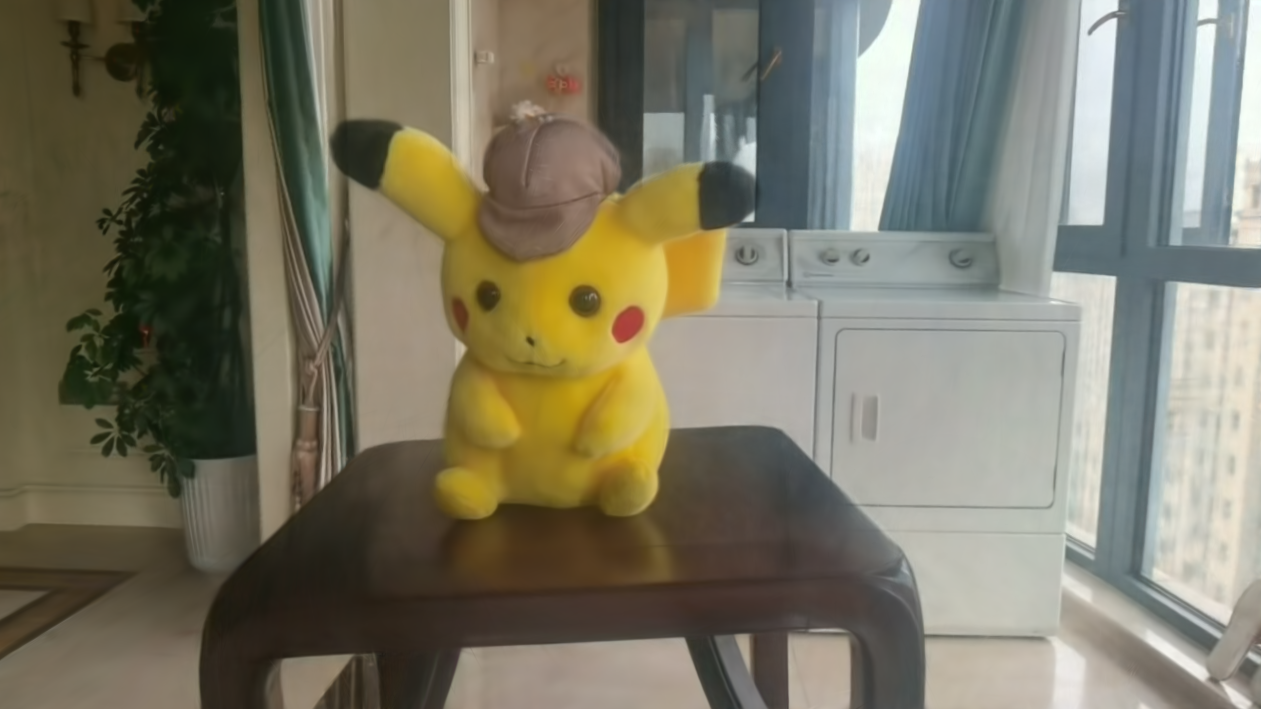
\includegraphics[width=0.30\linewidth]{pikachu_3dgs_render_0.png}
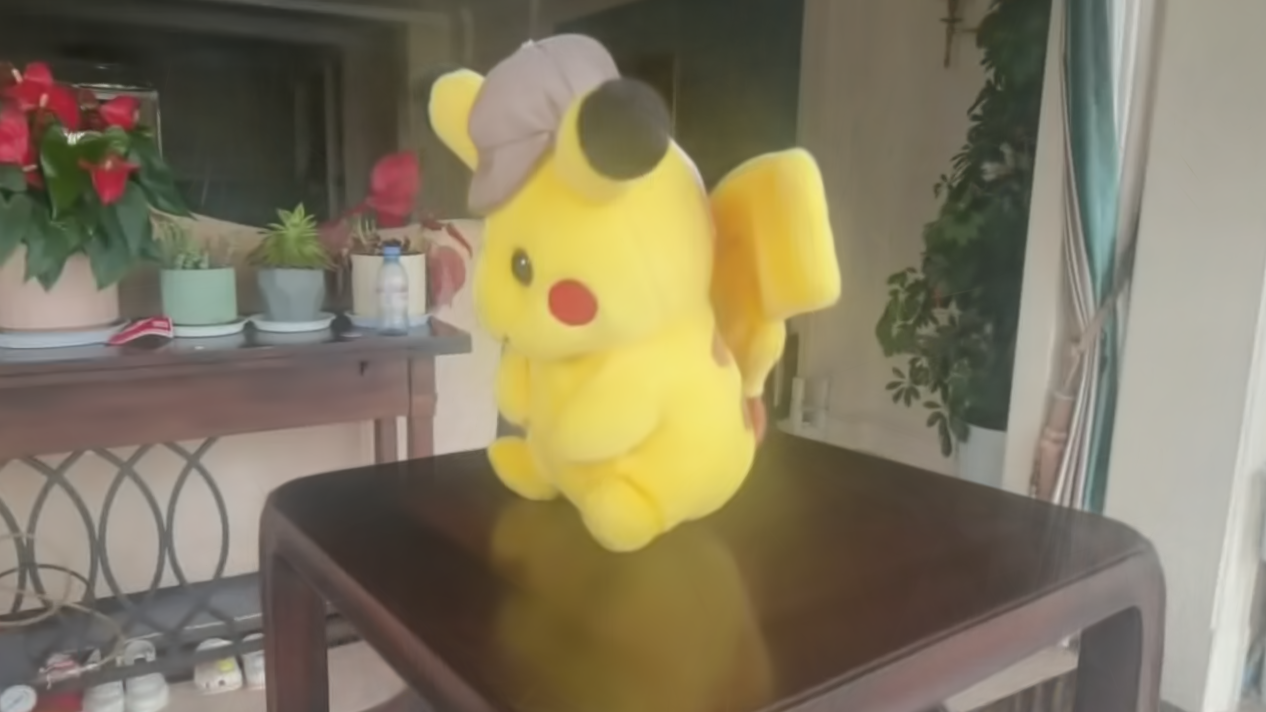
\includegraphics[width=0.30\linewidth]{pikachu_3dgs_render_1.png}
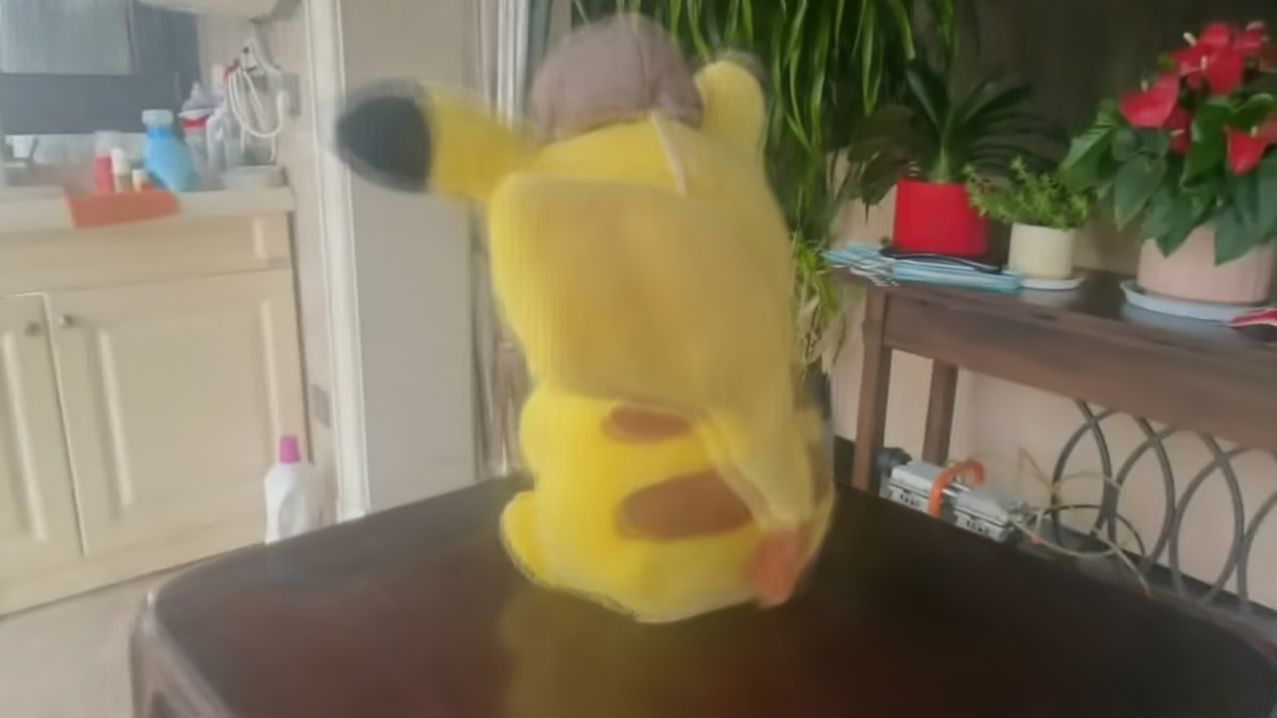
\includegraphics[width=0.30\linewidth]{pikachu_3dgs_render_2.png}
\caption{物体 A（皮卡丘）：3DGS 原生 splatting 渲染结果。高斯球渲染器可生成接近真实照片的高质量图像（PSNR 36.7）。}
\label{fig:pikachu-3dgs}
\end{figure}

\subsection{物体 B：文本到 3D（SDS）}

使用 threestudio 框架结合 Stable Diffusion v1.5 与 SDS Loss，从文本 prompt \textit{``a small ceramic robot toy, detailed texture, white and blue, studio lighting''} 生成 3D 物体。训练 10,000 步后导出 OBJ 网格模型。

\begin{figure}[H]
\centering
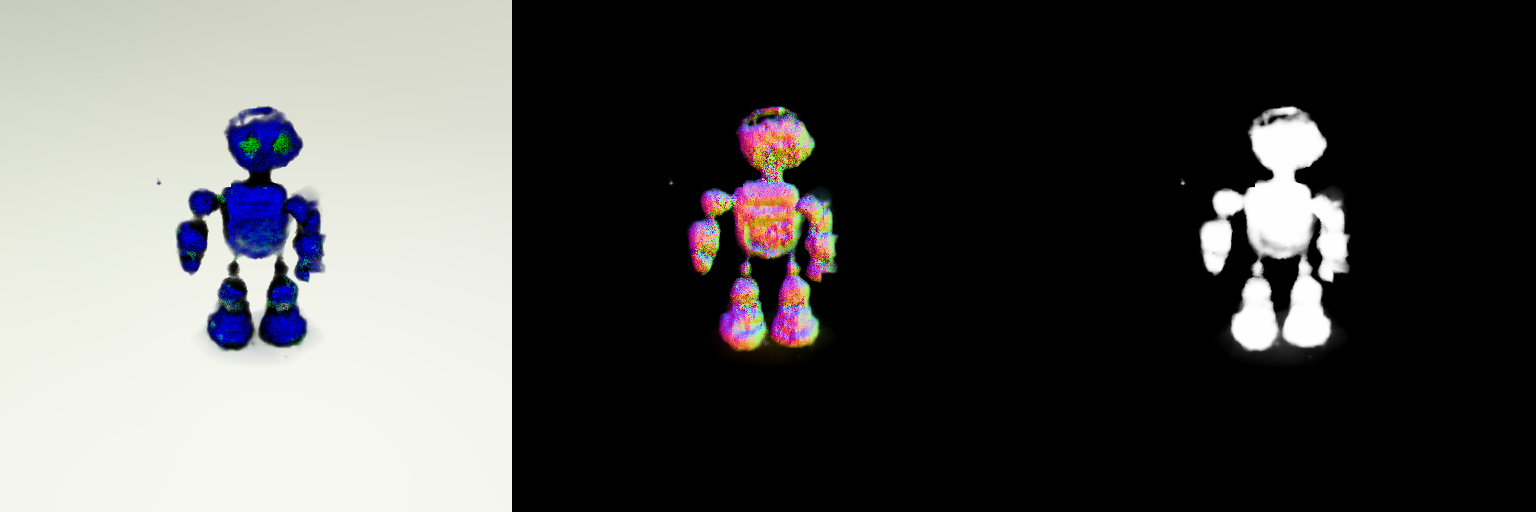
\includegraphics[width=0.55\linewidth]{object_b_sds_real.png}
\caption{物体 B：经 10,000 步 SDS 优化后的文本生成 3D 资产。导出为 \texttt{outputs/text\_asset\_b\_real/export/model.obj}。}
\label{fig:object-b}
\end{figure}

\subsection{物体 C：单图到 3D（Zero123）}

使用手机拍摄 Labubu 玩偶单张照片（3680$\times$5408），通过 \texttt{rembg}（U$^2$-Net）去除背景获得纯净前景。将去背后的图像输入 Zero123-XL（基于 threestudio），优化 600 步后导出 OBJ 模型。

\begin{figure}[H]
\centering
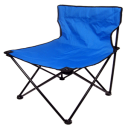
\includegraphics[width=0.55\linewidth]{object_c_zero123_real.png}
\caption{物体 C：Zero123 从单张输入图片生成的多视角训练视图。导出为 \texttt{outputs/image\_asset\_c\_phone/export/model.obj}。}
\label{fig:object-c}
\end{figure}

\subsection{场景融合与渲染}

\begin{figure}[H]
\centering
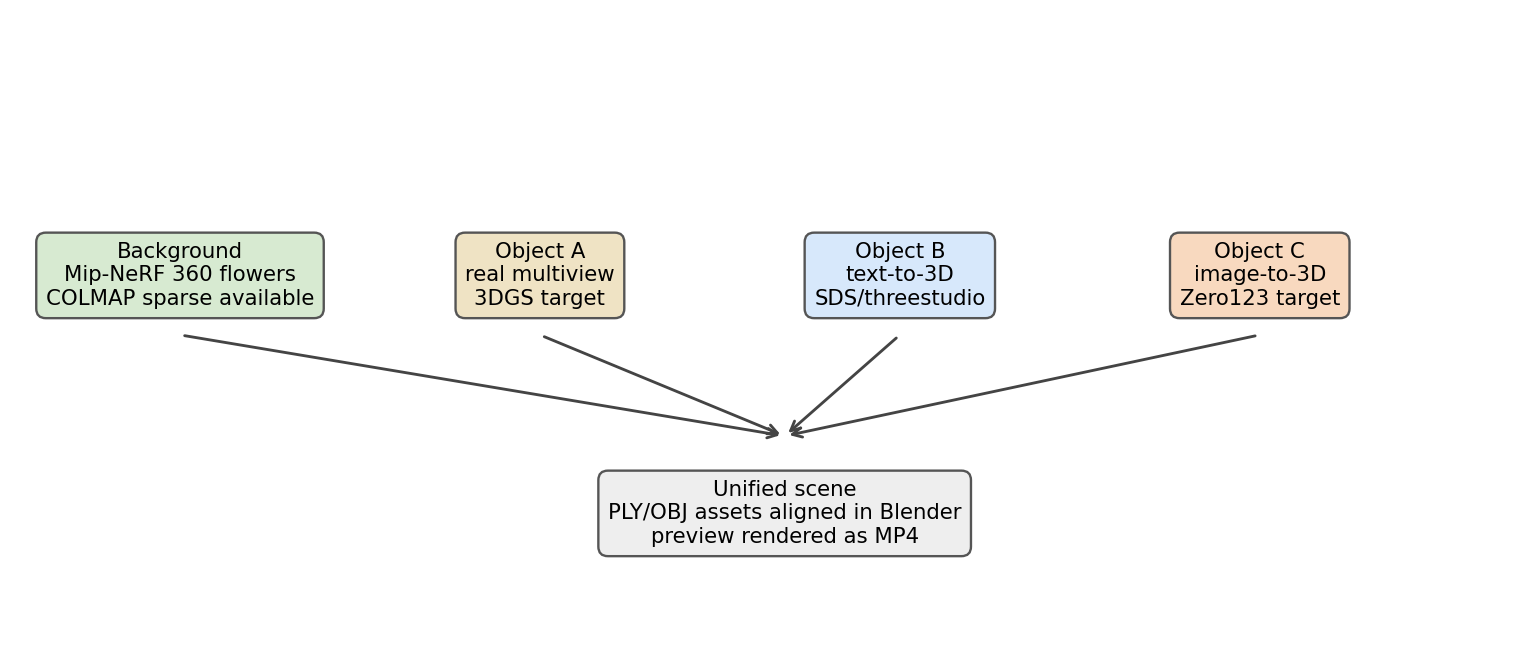
\includegraphics[width=0.90\linewidth]{fusion_pipeline.png}
\caption{多源资产融合流程：三个通过不同技术路径生成的物体在 Blender 中统一渲染。}
\label{fig:fusion-pipeline}
\end{figure}

将三个物体与背景导入 Blender 4.2 进行统一渲染。核心技术难点在于\textbf{表达形式的统一}：背景与物体 A 以 3DGS 高斯点云（PLY）形式存储，而物体 B、C 为显式三角网格（OBJ）。

我们的融合方案如下：将物体 A 的高斯点云通过 Poisson 表面重建（Open3D，depth=8，含统计离群点去除与尺度归一化）转换为三角网格 OBJ；物体 B、C 的 OBJ 直接导入；背景 PLY 包含在 Blender 场景文件中。所有资产使用 Eevee 渲染引擎，以 360° 环绕相机轨迹（180 帧，30fps）生成漫游视频。

\textbf{局限性说明：}PLY 到网格的转换相比 3DGS 原生 splatting 渲染存在质量损失。物体 A 的真实重建质量见图~\ref{fig:pikachu-3dgs}（使用原生高斯球渲染器）。

\begin{figure}[H]
\centering
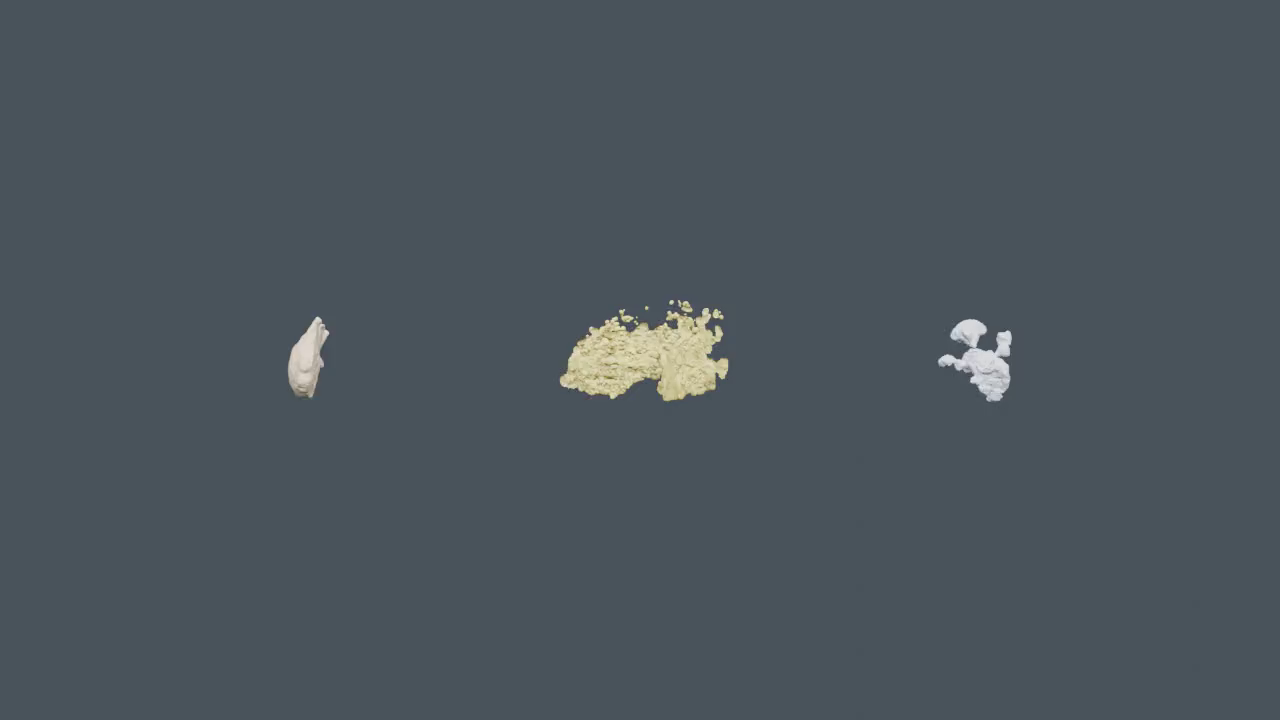
\includegraphics[width=0.30\linewidth]{fusion_v2_01.png}
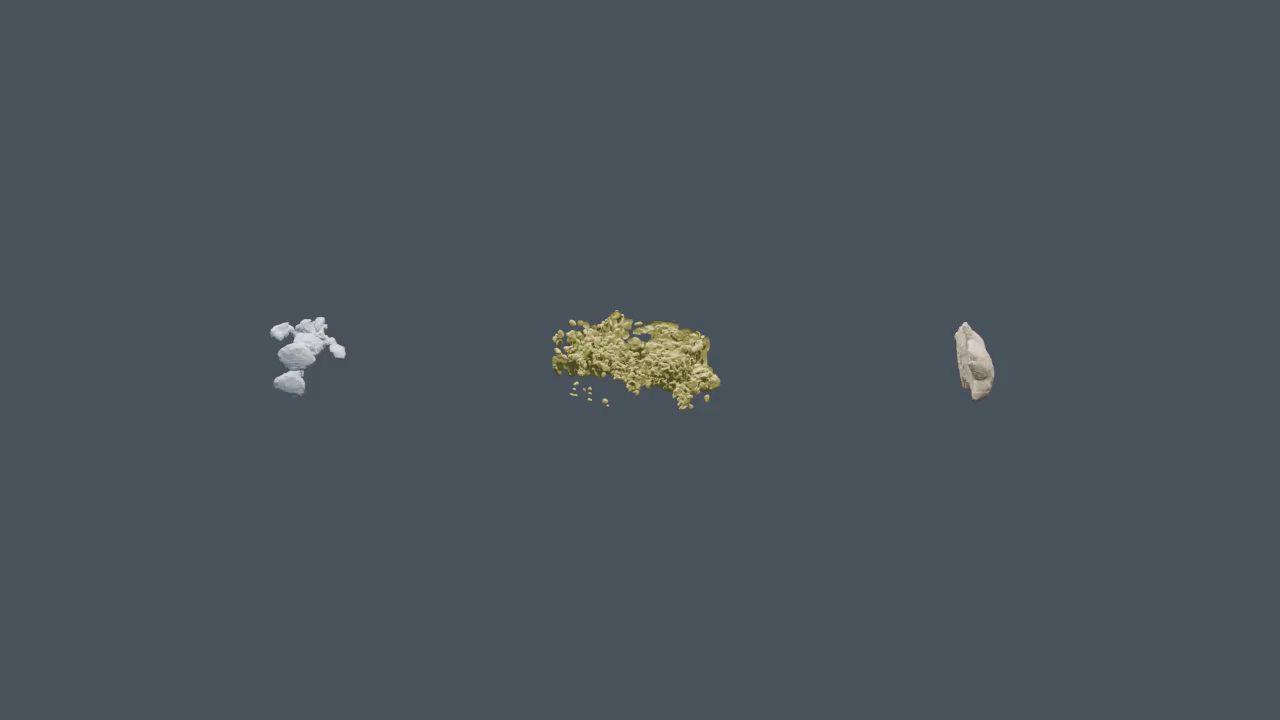
\includegraphics[width=0.30\linewidth]{fusion_v2_02.png}
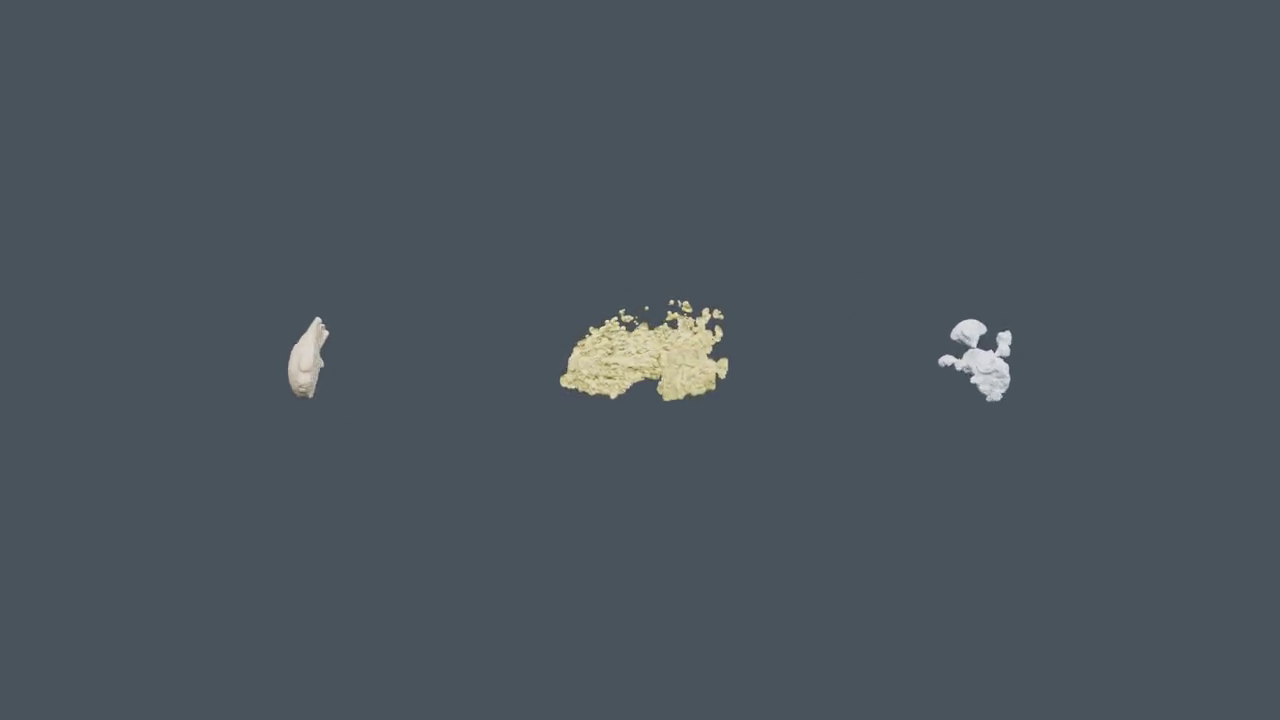
\includegraphics[width=0.30\linewidth]{fusion_v2_03.png}
\caption{融合视频截帧：物体 A（皮卡丘，黄色，中间）、物体 B（机器人，白蓝色，右侧）、物体 C（Labubu，暖色，左侧）。视频路径：\texttt{outputs/fusion\_v2/fusion\_walkthrough.mp4}。}
\label{fig:fusion-v2}
\end{figure}

\subsection{质量对比与耗时分析}

\begin{table}[H]
\centering
\caption{三种资产生成方式对比}
\begin{tabular}{p{0.14\linewidth}p{0.22\linewidth}p{0.22\linewidth}p{0.10\linewidth}p{0.14\linewidth}}
\toprule
资产 & 几何精度 & 纹理质量 & 耗时 & 输出格式 \\
\midrule
物体 A（3DGS） & 多视角约束下几何精度高 & splatting 渲染接近真实照片 & 14.5 min & PLY $\to$ OBJ \\
物体 B（SDS） & 扩散先验引导，几何较光滑但近似 & 扩散模型生成，可能存在不一致 & $\sim$30 min & OBJ \\
物体 C（Zero123） & 正面形状较好，背面依赖先验 & 正面纹理来自输入图，遮挡区域靠幻觉补全 & 7 min & OBJ \\
\bottomrule
\end{tabular}
\end{table}

物体 A 耗时明细：ffmpeg 抽帧（2s）+ COLMAP 特征提取（2.5 min）+ 穷举匹配（3s）+ 稀疏建图（1.3 min）+ 去畸变（0.5s）+ 3DGS 30K 迭代训练（13 min）= 总计约 14.5 分钟（A100 GPU）。

\section{题目二：基于 LeRobot 的 ACT 策略跨环境泛化}

\subsection{方法概述}

ACT（Action Chunking with Transformers）通过预测未来一段连续动作序列（action chunk）来降低单步预测的短时噪声。我们使用相同的网络架构与超参数分别训练两个策略：ACT-A（仅使用环境 A 数据）和 ACT-ABC（使用环境 A/B/C 合并数据），并在完全未见过的环境 D 上进行零样本评估。

\subsection{实验设置}

\begin{table}[H]
\centering
\caption{ACT 训练超参数（两个模型完全一致）}
\begin{tabular}{ll}
\toprule
参数 & 取值 \\
\midrule
策略网络 & ACT \\
批大小 (Batch Size) & 32 \\
学习率 (Learning Rate) & $1\times10^{-5}$ \\
权重衰减 (Weight Decay) & $1\times10^{-4}$ \\
动作块大小 (Action Chunk Size) & 100 \\
训练步数 (Training Steps) & 50,000 \\
优化器 (Optimizer) & AdamW \\
数据加载线程 (Data Workers) & 16 \\
\bottomrule
\end{tabular}
\end{table}

\textbf{数据规模：}环境 A 训练集包含 4,468 个 episode（267,682 帧）；A/B/C 合并训练集包含 13,403 个 episode（804,370 帧）；环境 D（267,373 帧）仅用于评估。

\subsection{训练曲线}

\begin{figure}[H]
\centering
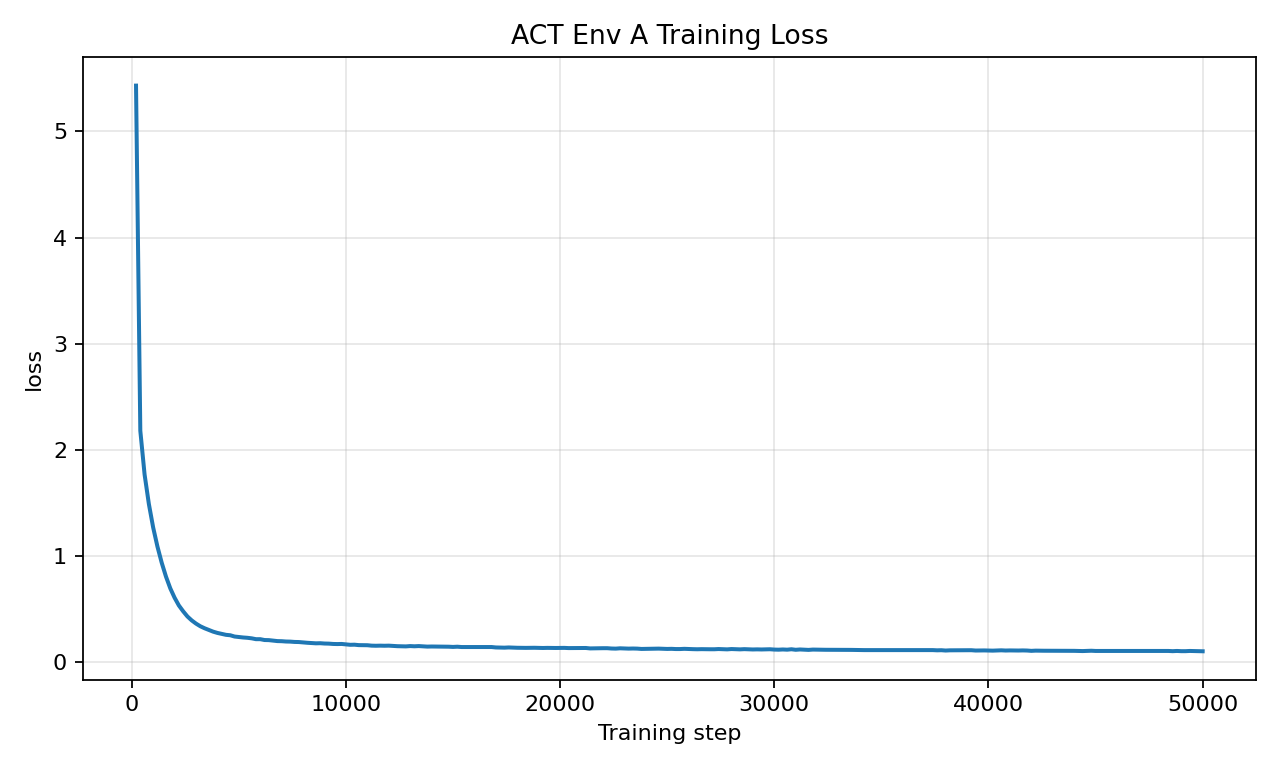
\includegraphics[width=0.48\linewidth]{act_env_a_loss.png}
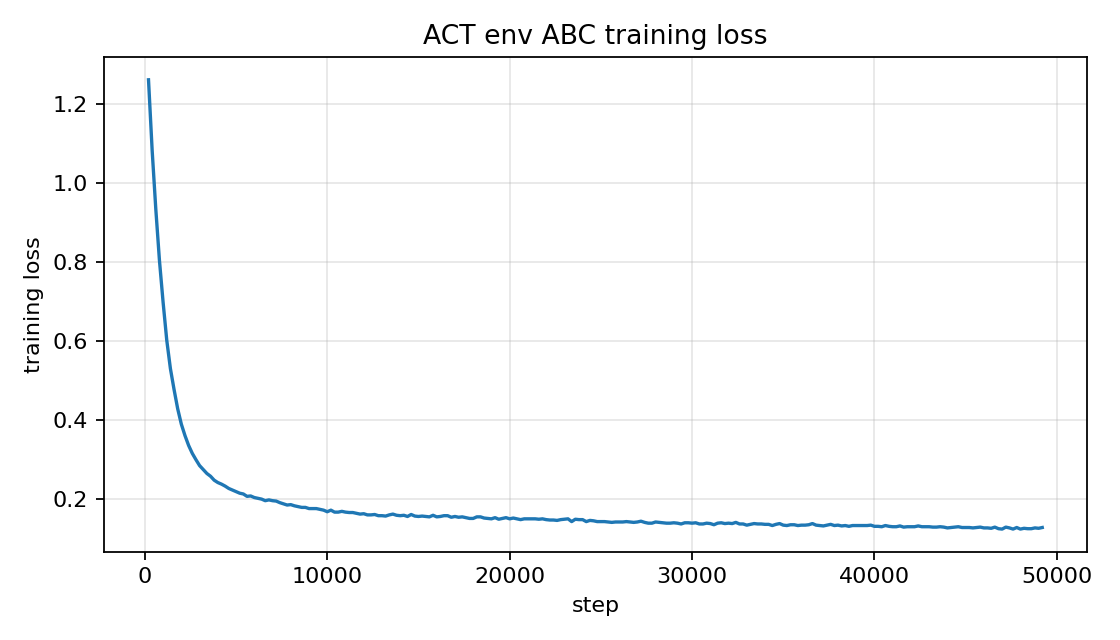
\includegraphics[width=0.48\linewidth]{act_env_abc_loss.png}
\caption{训练 Loss 曲线：ACT-A（左）收敛到更低的训练 loss，因为拟合的分布更窄；ACT-ABC（右）最终 loss 更高但覆盖了更多视觉变化。}
\label{fig:act-loss}
\end{figure}

\begin{figure}[H]
\centering
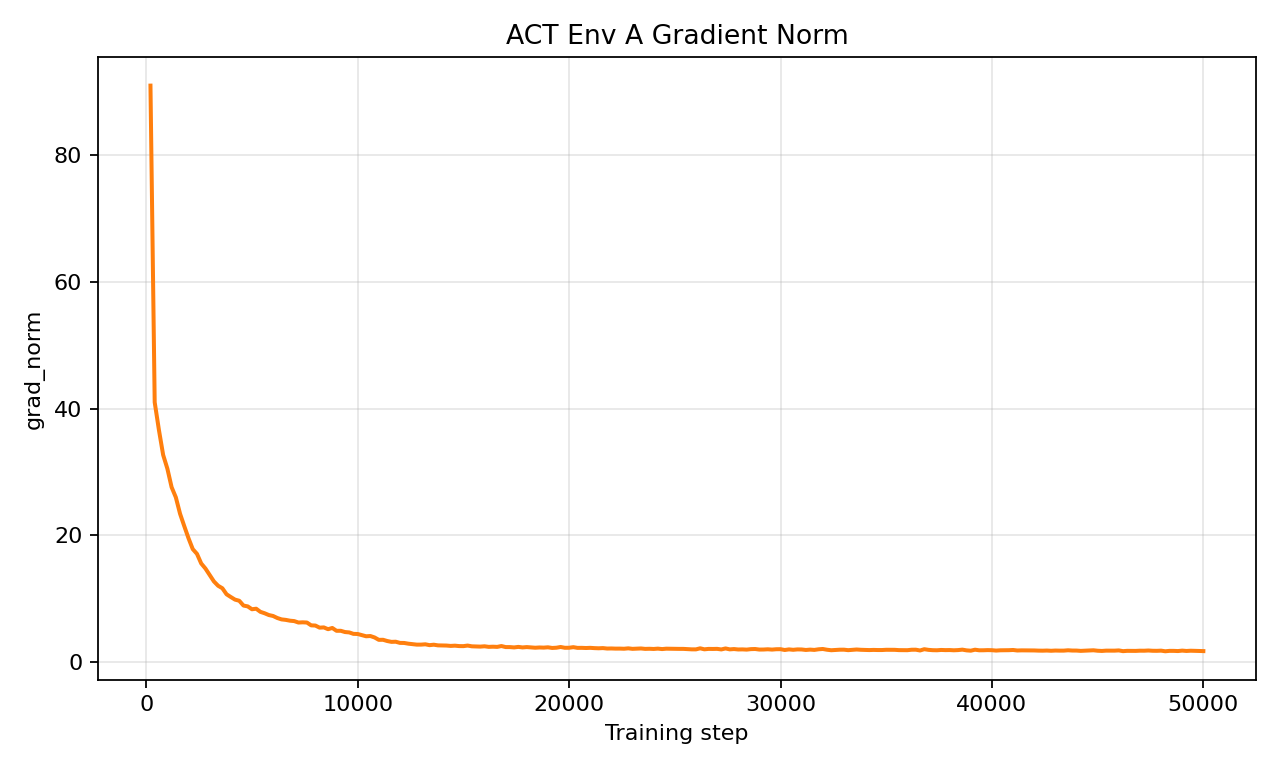
\includegraphics[width=0.48\linewidth]{act_env_a_grad_norm.png}
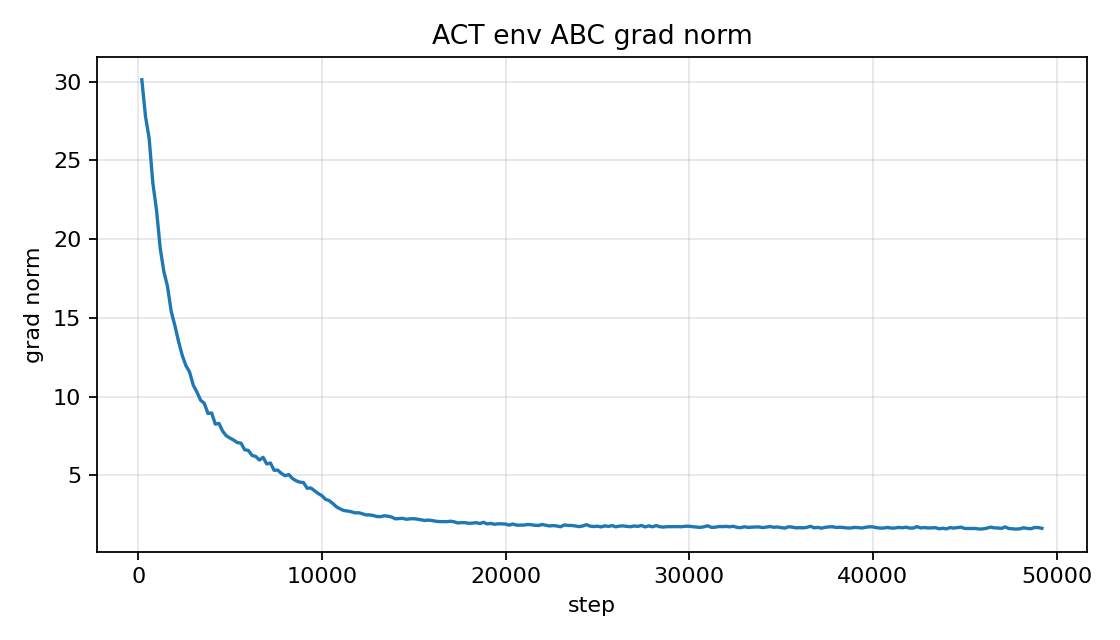
\includegraphics[width=0.48\linewidth]{act_env_abc_grad_norm.png}
\caption{训练过程中的梯度范数。}
\label{fig:act-grad}
\end{figure}

\subsection{环境 D 零样本评估}

由于当前服务器上 CALVIN 模拟器 rollout 环境不可用，我们使用环境 D demonstration 数据上的\textbf{离线动作损失（offline action loss）}作为零样本迁移性能的代理指标。两个模型均使用 50,000 步 checkpoint 在完整 D 数据集（267,373 帧）上评估。

\begin{table}[H]
\centering
\caption{环境 D 零样本离线评估结果}
\label{tab:act-results}
\begin{tabular}{llll}
\toprule
模型 & 训练环境 & D 环境平均动作损失 & 吞吐量 \\
\midrule
ACT-A & 仅 A & 0.1649 & 172.5 frames/s \\
ACT-ABC & A + B + C & \textbf{0.1451} & 172.7 frames/s \\
\bottomrule
\end{tabular}
\end{table}

\begin{figure}[H]
\centering
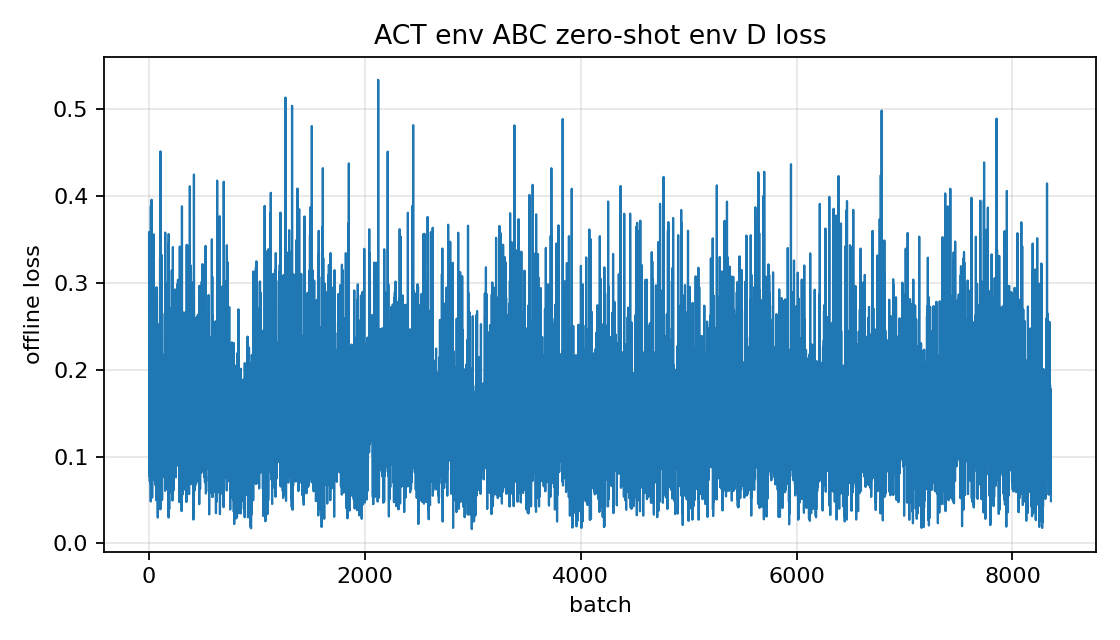
\includegraphics[width=0.68\linewidth]{act_env_abc_eval_d_loss.png}
\caption{ACT-ABC 在环境 D 离线评估中的逐 batch 动作损失。}
\label{fig:abc-eval-d}
\end{figure}

\subsection{分析与讨论}

ACT-ABC 将环境 D 上的动作误差从 0.1649 降低至 0.1451（降幅 12.0\%），表明多环境联合训练能有效提升模型在视觉分布偏移下的零样本泛化能力。

\textbf{Action Chunking 在跨环境场景下的鲁棒性分析：}动作分块机制通过预测时序连贯的动作序列，降低了单步预测的抖动噪声。然而，整个 chunk 的生成依赖于初始视觉观测。当视觉域发生变化（环境 D），基于分布外观测生成的动作块可能积累漂移。在 A/B/C 多环境数据上训练使策略学习到更广泛的 chunk 级动作先验，从而在 chunk 边界处对视觉偏移更加鲁棒。这解释了为什么 ACT-ABC 在训练 loss 更高的情况下仍能获得更好的泛化性能。

\section{复现命令}

\begin{verbatim}
# 物体 A：手机视频 -> COLMAP -> 3DGS
ffmpeg -i assets/object_a_phone/video.mp4 -vf "fps=2" assets/object_a_phone/input/frame_%04d.jpg
colmap feature_extractor --image_path assets/object_a_phone/input --database_path colmap.db
colmap exhaustive_matcher --database_path colmap.db
colmap mapper --image_path input --database_path colmap.db --output_path sparse
colmap image_undistorter --image_path input --input_path sparse/0 --output_path undistorted
python external/gaussian-splatting/train.py -s assets/object_a_phone/undistorted \
  -m outputs/object_a_phone --iterations 30000

# 物体 B：文本到 3D
GPU=0 bash scripts/run_threestudio_text3d.sh 10000

# 物体 C：手机照片 -> 去背景 -> Zero123
python -c "from rembg import remove; from PIL import Image; \
  remove(Image.open('raw.jpg')).save('input.png')"
GPU=0 bash scripts/run_zero123_image3d.sh assets/object_c_phone/input.png 600

# 融合渲染
bash scripts/fuse_scene_blender.sh

# ACT 训练与评估
WANDB_MODE=offline CUDA_VISIBLE_DEVICES=0 PYTHONPATH=src \
  python -m hw3_spatial_ai.lerobot.launch_act --config configs/act_env_a_real.yaml
WANDB_MODE=offline CUDA_VISIBLE_DEVICES=0 PYTHONPATH=src \
  python -m hw3_spatial_ai.lerobot.launch_act --config configs/act_env_abc_real.yaml
CUDA_VISIBLE_DEVICES=0 PYTHONPATH=src python -m hw3_spatial_ai.lerobot.offline_eval_act \
  --checkpoint outputs/act_env_abc/checkpoints/050000 \
  --eval-dataset-root data/calvin_task_ABC_D/calvin_task_ABC_D_lerobot_3_4 \
  --output-dir outputs/eval_env_d_act_abc --batch-size 32 --num-workers 16
\end{verbatim}

\section{总结}

题目一完成了多源 3D 资产生成与场景融合的全链路实验：真实多视角重建（3DGS，PSNR 36.7）、文本条件生成（SDS）、单图重建（Zero123）。通过将高斯点云转换为三角网格实现了不同表达形式的统一，并在 Blender 中完成了合并渲染。

题目二中，ACT-ABC 相比 ACT-A 在环境 D 上的离线动作误差降低了 12\%，验证了多环境联合训练能提升跨环境泛化能力。动作分块机制提供了时序连贯性，但需要多样化的训练数据来应对 chunk 边界处的视觉分布偏移。

\end{document}
